%%%%%%%%%%%%%%%%%%%%%%%%%%%%%%%%%%%%%%%%%
% baposter Landscape Poster
% LaTeX Template
% Version 1.0 (11/06/13)
%
% baposter Class Created by:
% Brian Amberg (baposter@brian-amberg.de)
%
% This template has been downloaded from:
% http://www.LaTeXTemplates.com
%
% License:
% CC BY-NC-SA 3.0 (http://creativecommons.org/licenses/by-nc-sa/3.0/)
%
%%%%%%%%%%%%%%%%%%%%%%%%%%%%%%%%%%%%%%%%

% Sections:
% 	- SAGA
% 	- RP
% 	- ENMD
% 	- How to use RADICAL-Cybertools
% 	- Who uses RADICAL-Cybertools
	% - EXTASY
	% - REPEX









%----------------------------------------------------------------------------------------
%	PACKAGES AND OTHER DOCUMENT CONFIGURATIONS
%----------------------------------------------------------------------------------------

\documentclass[landscape,a0paper,fontscale=0.285]{baposter} % Adjust the font scale/size here

\usepackage{graphicx} % Required for including images
\graphicspath{{figures/}} % Directory in which figures are stored

\usepackage{amsmath} % For typesetting math
\usepackage{amssymb} % Adds new symbols to be used in math mode

\usepackage{booktabs} % Top and bottom rules for tables
\usepackage{enumitem} % Used to reduce itemize/enumerate spacing
\usepackage{palatino} % Use the Palatino font
\usepackage[font=small,labelfont=bf]{caption} % Required for specifying captions to tables and figures

\usepackage{multicol} % Required for multiple columns
\setlength{\columnsep}{1.5em} % Slightly increase the space between columns
\setlength{\columnseprule}{0mm} % No horizontal rule between columns

\usepackage{tikz} % Required for flow chart
\usetikzlibrary{shapes,arrows} % Tikz libraries required for the flow chart in the template

\newcommand{\compresslist}{ % Define a command to reduce spacing within itemize/enumerate environments, this is used right after \begin{itemize} or \begin{enumerate}
\setlength{\itemsep}{1pt}
\setlength{\parskip}{0pt}
\setlength{\parsep}{0pt}
}

\definecolor{lightblue}{rgb}{0.145,0.6666,1} % Defines the color used for content box headers

\begin{document}

\begin{poster}
{
headerborder=closed, % Adds a border around the header of content boxes
colspacing=1em, % Column spacing
bgColorOne=white, % Background color for the gradient on the left side of the poster
bgColorTwo=white, % Background color for the gradient on the right side of the poster
borderColor=lightblue, % Border color
headerColorOne=black, % Background color for the header in the content boxes (left side)
headerColorTwo=lightblue, % Background color for the header in the content boxes (right side)
headerFontColor=white, % Text color for the header text in the content boxes
boxColorOne=white, % Background color of the content boxes
textborder=roundedleft, % Format of the border around content boxes, can be: none, bars, coils, triangles, rectangle, rounded, roundedsmall, roundedright or faded
eyecatcher=true, % Set to false for ignoring the left logo in the title and move the title left
headerheight=0.1\textheight, % Height of the header
headershape=roundedright, % Specify the rounded corner in the content box headers, can be: rectangle, small-rounded, roundedright, roundedleft or rounded
headerfont=\Large\bf\textsc, % Large, bold and sans serif font in the headers of content boxes
%textfont={\setlength{\parindent}{1.5em}}, % Uncomment for paragraph indentation
linewidth=2pt % Width of the border lines around content boxes
}
%----------------------------------------------------------------------------------------
%	TITLE SECTION 
%----------------------------------------------------------------------------------------
%
{
\includegraphics[height=4em]{logo.png}} % First university/lab logo on the left
{\bf\textsc{RADICAL-Cybertools: An Overview}\vspace{0.5em}} % Poster title
{\textsc{\{ John Smith, James Smith and Jane Smith \} \hspace{12pt} University and Department Name}} % Author names and institution
{
\includegraphics[height=4em]{logo.png}} % Second university/lab logo on the right

%----------------------------------------------------------------------------------------
%	OBJECTIVES
%----------------------------------------------------------------------------------------

\headerbox{What does RADICAL do?}{name=objectives,column=0,row=0}{
RADICAL Cybertools is a collections abstraction-based tools that are architected for scalable, interoperable and sustainable operations on high-performance and distributed computing systems. The three main components of the suite are:

\begin{itemize}\compresslist
\item RADICAL-SAGA 
\item RADICAL-Pilot (RP)
\item EnsembleMD Toolkit
\end{itemize}

The RADICAL group develops these components as open source projects with the goal of providing application level control over high-performance resources, as in the case of RP, and abstracting common tasks and patterns across those resources, as in the case of EnsembleMD. The Cybertools account for the heterogeniety of distributed computing resources (DCRs) and expose simple interfaces to the user for work at various levels (rephrase?).

\vspace{0.3em} % When there are two boxes, some whitespace may need to be added if the one on the right has more content
}

%----------------------------------------------------------------------------------------
%	INTRODUCTION
%----------------------------------------------------------------------------------------

\headerbox{Why Pilots?}{name=introduction,column=1,row=0,bottomaligned=objectives}{
Currently, many scientific simulations are performed by submitting many similar executables to a DCR and then waiting for each to be scheduled, executed, and probed for output data. The time-to-completion for such simulations becomes impractical as the number of tasks increases, which hinders progress on those projects. To combat this, Pilot systems were introduced to obviate the need to schedule each task, and have the following properties:

\begin{itemize}\compresslist
\item Submitting only the Pilot to circumvent the scheduler.
\item Achieve spatial and temporal locality for related tasks.
\item Decreased time-to-completion.
\end{itemize}

% instead, only the Pilot, bearing the description of the requested resources and computational tasks, is scheduled to the machine and coordinates execution. The main benefit of this scheme is that the scheduler has essentially been circumvented, allowing the same number of tasks to be submitted with a drastically reduced time-to-completion. RADICAL-Cybertools leverage this advantage to create software to simplify and expedite simulation.

% and executing these is proportional to the number of simulations submitted, as each one must wait in the queue and be scheduled individually. The time-to-completion of these tasks becomes extended due to this, causing large experiments to run for undesirable lengths of time. Furthermore, the resources granted to each simulation may not allocated in an efficient way; for example, some instances may be MPI-based and depend on the proximity of one simulation's cores to another's. The Pilot was invented to assuage these issues.

}

%----------------------------------------------------------------------------------------
%	RESULTS 1
%----------------------------------------------------------------------------------------

\headerbox{Projects}{name=results,column=2,span=2,row=0}{

\begin{multicols}{2}
\vspace{1em}
\begin{center}
\includegraphics[width=0.8\linewidth]{enmd_flow}
\captionof{figure}{The EnsembleMD Architecture}
\end{center}
The EnsembleMD Toolkit consists of a series of Execution Patterns and Kernels that provide a simple interface for running high-performance tasks on a distributed computing resource (DCR). Using the API, a user can avoid placing each task into the queue by specifying the target machine through the Execution Context interface, the simulation through the Kernel interface, and the Execution Pattern through the Pattern interface. Once these entities are specified, the RADICAL-Pilot API is invoked to translate the descriptions into a Pilot and its associated Compute Units, and then to execute the simulations on the desired resource. 
\end{multicols}

%------------------------------------------------

\begin{multicols}{2}
\vspace{1em}
Users of RADICAL-Pilot (RP) interact with the API by describing Compute Units, which represent the task, and a Pilot. Once instantiated and described, the Pilot is submitted to the Pilot Manager and the Compute Unit is submitted to the Unit Manager. These entities manage the launching of the Pilot and Compute Units onto the Distributed Computing Resources, where the Pilot Agent is instantiated and carries out the execution of the tasks.
\begin{center}
\includegraphics[width=0.8\linewidth]{rp_flow}
\captionof{figure}{The RADICAL-Pilot Architecture}
\end{center}

\end{multicols}
}

%----------------------------------------------------------------------------------------
%	REFERENCES
%----------------------------------------------------------------------------------------

\headerbox{References}{name=references,column=0,above=bottom}{

\renewcommand{\section}[2]{\vskip 0.05em} % Get rid of the default "References" section title
\nocite{*} % Insert publications even if they are not cited in the poster
\small{ % Reduce the font size in this block
\bibliographystyle{unsrt}
\bibliography{sample} % Use sample.bib as the bibliography file
}}

%----------------------------------------------------------------------------------------
%	FUTURE RESEARCH
%----------------------------------------------------------------------------------------

\headerbox{Future Research}{name=futureresearch,column=1,span=2,aligned=references,above=bottom}{ % This block is as tall as the references block

\begin{multicols}{2}
Integer sed lectus vel mauris euismod suscipit. Praesent a est a est ultricies pellentesque. Donec tincidunt, nunc in feugiat varius, lectus lectus auctor lorem, egestas molestie risus erat ut nibh.

Maecenas viverra ligula a risus blandit vel tincidunt est adipiscing. Suspendisse mollis iaculis sem, in \emph{imperdiet} orci porta vitae. Quisque id dui sed ante sollicitudin sagittis.
\end{multicols}
}

%----------------------------------------------------------------------------------------
%	CONTACT INFORMATION
%----------------------------------------------------------------------------------------

\headerbox{Contact Information}{name=contact,column=3,aligned=references,above=bottom}{ % This block is as tall as the references block

\begin{description}\compresslist
\item[Web] radical.rutgers.edu
\item[RP Docs] http://radicalpilot.readthedocs.org/en/latest/ 
\item[EnsembleMD Docs]b http://radicalensemblemd.readthedocs.org/en/latest/ 
\end{description}
}

%----------------------------------------------------------------------------------------
%	CONCLUSION
%----------------------------------------------------------------------------------------

\headerbox{Additional Projects}{name=conclusion,column=2,span=2,row=0,below=results,above=references}{
(AIMES, etc.)


% \begin{multicols}{2}

% % \tikzstyle{decision} = [diamond, draw, fill=blue!20, text width=4.5em, text badly centered, node distance=2cm, inner sep=0pt]
% % \tikzstyle{block} = [rectangle, draw, fill=blue!20, text width=5em, text centered, rounded corners, minimum height=4em]
% % \tikzstyle{line} = [draw, -latex']
% % \tikzstyle{cloud} = [draw, ellipse, fill=red!20, node distance=3cm, minimum height=2em]

% % \begin{tikzpicture}[node distance = 2cm, auto]
% % \node [block] (init) {Initialize Model};
% % \node [cloud, left of=init] (Start) {Start};
% % \node [cloud, right of=init] (Start2) {Start Two};
% % \node [block, below of=init] (init2) {Initialize Two};
% % \node [decision, below of=init2] (End) {End};
% % \path [line] (init) -- (init2);
% % \path [line] (init2) -- (End);
% % \path [line, dashed] (Start) -- (init);
% % \path [line, dashed] (Start2) -- (init);
% % \path [line, dashed] (Start2) |- (init2);
% % \end{tikzpicture}

% %------------------------------------------------

% \begin{itemize}\compresslist
% \item Pellentesque eget orci eros. Fusce ultricies, tellus et pellentesque fringilla, ante massa luctus libero, quis tristique purus urna nec nibh. Phasellus fermentum rutrum elementum. Nam quis justo lectus.
% \item Vestibulum sem ante, hendrerit a gravida ac, blandit quis magna.
% \end{itemize}

% \end{multicols}
}

%----------------------------------------------------------------------------------------
%	MATERIALS AND METHODS
%----------------------------------------------------------------------------------------

\headerbox{Using RADICAL-Pilot (RP)}{name=method,column=0,below=objectives,bottomaligned=conclusion}{ % This block's bottom aligns with the bottom of the conclusion block


\begin{center}
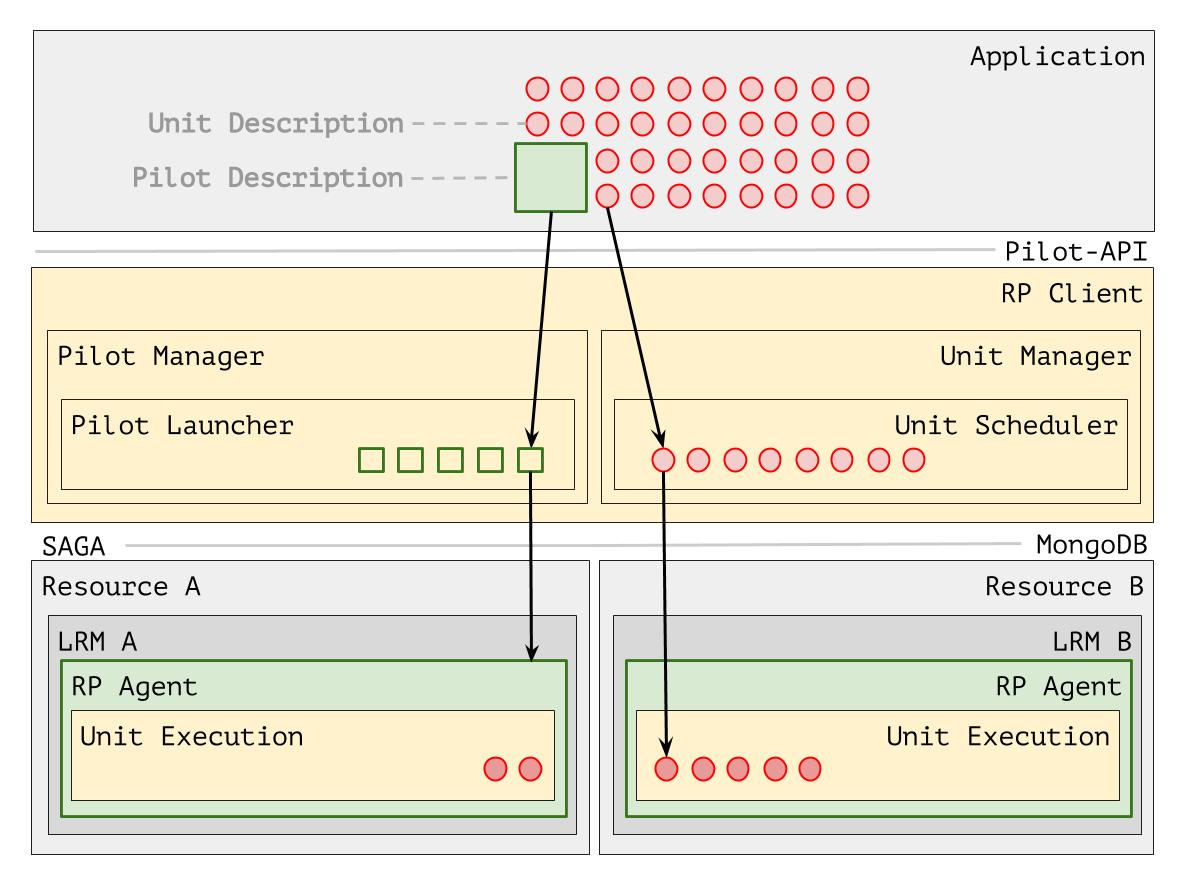
\includegraphics[width=0.7\linewidth]{rp_arch}
\captionof{figure}{Figure caption}
\end{center}




% The following materials were required to complete the research:

% \begin{itemize}\compresslist
% \item Curabitur pellentesque dignissim
% \item Eu facilisis est tempus quis
% \item Duis porta consequat lorem
% \item Eu facilisis est tempus quis
% \end{itemize}

% The following equations were used for statistical analysis:

% \begin{equation}
% \cos^3 \theta =\frac{1}{4}\cos\theta+\frac{3}{4}\cos 3\theta
% \label{eq:refname}
% \end{equation}\

% \begin{equation}
% E = mc^{2}
% \label{eqn:Einstein}
% \end{equation}

% Phasellus imperdiet, tortor vitae congue bibendum, felis enim sagittis lorem, et volutpat ante orci sagittis mi. Morbi rutrum laoreet semper. Morbi accumsan enim nec tortor consectetur non commodo nisi sollicitudin. Proin sollicitudin. Pellentesque eget orci eros. Fusce ultricies, tellus et pellentesque fringilla, ante massa luctus libero, quis tristique purus urna nec nibh.
}

%----------------------------------------------------------------------------------------
%	RESULTS 2http://radicalensemblemd.readthedocs.org/en/latest/http://radicalensemblemd.readthedocs.org/en/latest/
%----------------------------------------------------------------------------------------

\headerbox{Who uses the Cybertools?}{name=results2,column=1,below=objectives,bottomaligned=conclusion}{ % This block's bottom aligns with the bottom of the conclusion block

A number of groups around the globe use RADICAL-Cybertools. Some of our current collaborators are:

RADICAL-SAGA
\begin{itemize}\compresslist
\item Atlas Experiment
\item Super Kamiokande
\end{itemize}

RADICAL-Pilot
\begin{itemize}\compresslist
\item Replica Exchange
\item EnsembleMD Toolkit
\end{itemize}



% \begin{center}
% \begin{tabular}{l l l}
% \toprulehttp://radicalensemblemd.readthedocs.org/en/latest/
% \textbf{Treatments} & \textbf{Response 1} & \textbf{Response 2}\\
% \midrule
% Treatment 1 & 0.0003262 & 0.562 \\
% Treatment 2 & 0.0015681 & 0.910 \\
% Treatment 3 & 0.0009271 & 0.296 \\
% \bottomrule
% \end{tabular}
% \captionof{table}{Table caption}
% \end{center}

% Nulla ut porttitor enim. Suspendisse venenatis dui eget eros gravida tempor. Mauris feugiat elit et augue placerat ultrices. Morbi accumsan enim nec tortor consectetur non commodo.

% \begin{center}
% \begin{tabular}{l l l}
% \toprule
% \textbf{Treatments} & \textbf{Response 1} & \textbf{Response 2}\\
% \midrule
% Treatment 1 & 0.0003262 & 0.562 \\
% Treatment 2 & 0.0015681 & 0.910 \\
% Treatment 3 & 0.0009271 & 0.296 \\
% \bottomrule
% \end{tabular}
% \captionof{table}{Table caption}
% \end{center}
}

%----------------------------------------------------------------------------------------

\end{poster}

\end{document}